% Artifact mockup only. Not input by main.tex.
% Table 17 (adjusted origin contrasts) remains in the manuscript.
\documentclass[11pt]{article}
\usepackage[margin=1in]{geometry}
\usepackage[utf8]{inputenc}
\usepackage[T1]{fontenc}
\usepackage{mathptmx}
\usepackage{graphicx}
\usepackage{microtype}
\usepackage[font=small,labelfont=bf,labelsep=period]{caption}

\begin{document}
\pagestyle{empty}

\noindent\textit{Mockup page (not in the manuscript PDF). Table~17 remains in the paper.}

\vspace{1.2em}

\begin{figure}[h]
\centering
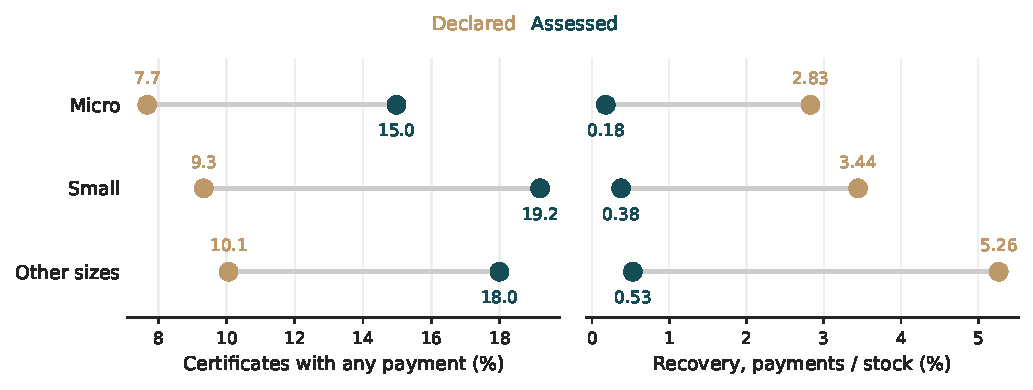
\includegraphics[width=\textwidth]{fig_origin_levels.pdf}
\caption{Declared and assessed certificates by firm size.
The left panel is the share of certificates with any payment.
The right panel is payments divided by December stock.
Each row is a firm-size group.
The warm marker is declared debt and the teal marker is assessed debt.
Unknown size is omitted because the assessed cell has one to four payers.
Across size groups, assessed debt has the higher payment rate and declared debt has the higher recovery rate.}
\end{figure}

\end{document}
